\documentclass[a4paper,10pt]{article}
\usepackage[utf8]{inputenc}
\usepackage{graphicx}    
\usepackage{color}
%\usepackage{epsfig}   
\usepackage[font=footnotesize]{subfig}
\usepackage{float}
\usepackage{fancyhdr}                              
\usepackage{makeidx}
\usepackage[nottoc,notlot,notlof]{tocbibind}     
\usepackage{supertabular}
\usepackage{array}              
\usepackage{setspace} 
\usepackage{enumerate}
\usepackage{rotating}
\usepackage{moreverb}
\usepackage{multirow}
\usepackage{amsmath}
\usepackage{amsthm}
\usepackage{amssymb}
\usepackage{captcont}
\usepackage{verbatim}
\usepackage{titlesec}
\usepackage{url}
\usepackage{hyperref}
\usepackage{lipsum}
\usepackage{tikz}
\usepackage{pgf-pie}
\usepackage{pgfplots}
\usepackage{array}
\usepackage{booktabs}
\usepackage{blindtext}
\usepackage{tabularx}
%\usepackage[utf8]{inputenc}
\usepackage{commath}

\newcolumntype{L}[1]{>{\raggedright\let\newline\\\arraybackslash\hspace{0pt}}m{#1}}
\usepackage[margin=1in]{geometry}
\begin{document}


\section{Results and Findings}



The analysis was performed for differnet timeseries of two centers- Delhi and Mumbai.

Following analysis is for Mumbai. In case of Mumbai, there are total of 66 distinct days for which news articles exist. Here, articles not matched represents unique dates for which articles were present but system failed to report anomaly against that date.
\begin{table}[H]
\centering

\begin{tabular}{| L{3cm} | L{3cm} | L{3cm} | L{3cm} | L{3cm} |}
\hline                                 
				  & \textbf{Anomalies \newline Reported} & \textbf{Anomalies \newline Matched}  & \textbf{Articles \newline Not Matched}   & \textbf{Articles Not Matched which stated traders nexus as reason} \\ \hline
\textbf{Retail Vs Average Retail} & 125                         & 64                          &  49                		&  12 (24.49\%)                \\ \hline
\textbf{Retail Vs Arrival}        & 323                         & 153                         &  33                		&  9  (27.27\%)              \\ \hline
\textbf{Retail Vs Wholesale}      & 160                         & 52                          &  52                		&  14 (26.92\%)               \\ \hline
\textbf{Wholesale Vs Arrival}     & 332                         & 168                         &  29                		&  7  (24.13\%)              \\ \hline
\end{tabular}
\caption{System Result for Mumbai}
\label{table:result}
\end{table}

Following are the inferences from the above table:
\begin{itemize}
 \item Analysis involving arrival timeseries tends to produce better matches. This could be because arrival is one of the determining factor for the price of commodity. Also, news often compare arrival data to explain the suspicous scenarios.
 \item Retail vs Average Retail does not produce good matches which shows that the prices at differnet centers tend to go in tendum which might be because of strong traders nexus.
 \item Retail vs Wholesale is not performing good results which gives a clear indication that usually retail prices align with the wholesale prices. So, retailers don't tend to get involved in the fixing of prices because they are forced to align the price of commodity with the wholesale prices.
 \item This also indirectly indicates that the most of the problem exists at the wholesale level where traders operate who are usually accused by the news reports for manipulating the price of commodity.
\end{itemize}

As shown in the above table \ref{table:result}, from the number of news articles which are missed by system, almost 25\% of them are of traders nexus. Rest 75\% are because of low production, unseasonal rainfall, low supply, etc. Now, one of the reason why these articles were missed may be because of arrival will be low during this tenure and it is normal to have price hike. So, that might be reason that system might have considered them as normal that prices are high. Usually news sources report in article whenever prices goes high, but system only detects anomalous cases.

\begin{table}[H]
	\centering	
	\begin{tabular}{|l|}
		\hline
		\textbf{Dates with article trader nexus missed by system} \\ \hline
		2012-12-27                                                \\ \hline
		2013-01-22                                                \\ \hline
		2013-01-30                                                \\ \hline
		2013-07-03                                                \\ \hline
		2014-06-20                                                \\ \hline
		2014-06-30                                                \\ \hline
		2014-07-01                                                \\ \hline
	\end{tabular}
	\caption{Common 7 Dates with article trader nexus missed by system}
	\label{table:missed7}
\end{table}

Now, the one which are stating traders nexus as reason, and are missed by system were studied. There are 7 cases which are common to all four type of analysis. These 7 dates are shown in table \ref{table:missed7}. Note that there exist 24 unique dates for which trader nexus articles are present. So 71\% of traders nexus article were reported by system overall. So, we tried to dig up why system missed them. On studying those cases, we found following:

\begin{itemize}

	\item When we looked for Retail vs Average Retail series, we found that all centers were behaving similar. Where as this analysis detects when one center deviates from other. That's why system might have missed them. One more point to note is that these articles are for traders nexus and it is quite common that traders will be communucating among themselves and controlling the prices and that is the reason why we observed that centers are behaving similar.
	
	\item For Retail vs Arrival analysis, Hypothesis 1 reported some of the anomalies, but Hypothesis 3 did not. Hypothesis reports anomalies date-wise and Hypothesis 1 reports anomalies window-wise. So, we found that while taking intersection these anomalies got removed. Note that in Hypothsis 3 not exact date, but nearby dates were reported.
	
	\item When we studied Retail vs Wholesale Analysis, we found that in all cases, both prices were moving hand in hand. So, this analysis could not capture these anomalies. \textbf{ Note that this might be the reason, why Retail vs Average Retail and Retail vs Wholesale are not producing promising results because they usually go hand in hand. But when arrival comes into picture, then we can have better estimate of prices. So analysis which is which arrival are performing better as compared to others}
	
	\item For Wholesale vs Arrival, 3 of the anomalies were reported by Hypothesis 1. But as stated above for Retail vs Arrival, here too Hypothesis 3 results could not report exact date and we missed them. For the remaining cases in this analysis, we could not find particular reason why they are not reported.
	
\end{itemize}

Following figures are the pictorical representation of the above results (See table \ref{table:result}) on timeline.

\textbf{Note:} In following figures, Yellow highlighted regions are system reported anomalies for which no corresponding news article was present, Grey highlighted region represents news article for which our system did not report any anomaly and Red highlighted region represents anomalies reported by system for which news articles were present.

\begin{itemize}
 \item Retail Price vs Average Retail Price
			
			\begin{figure}[H]
		    	\centering
  		    	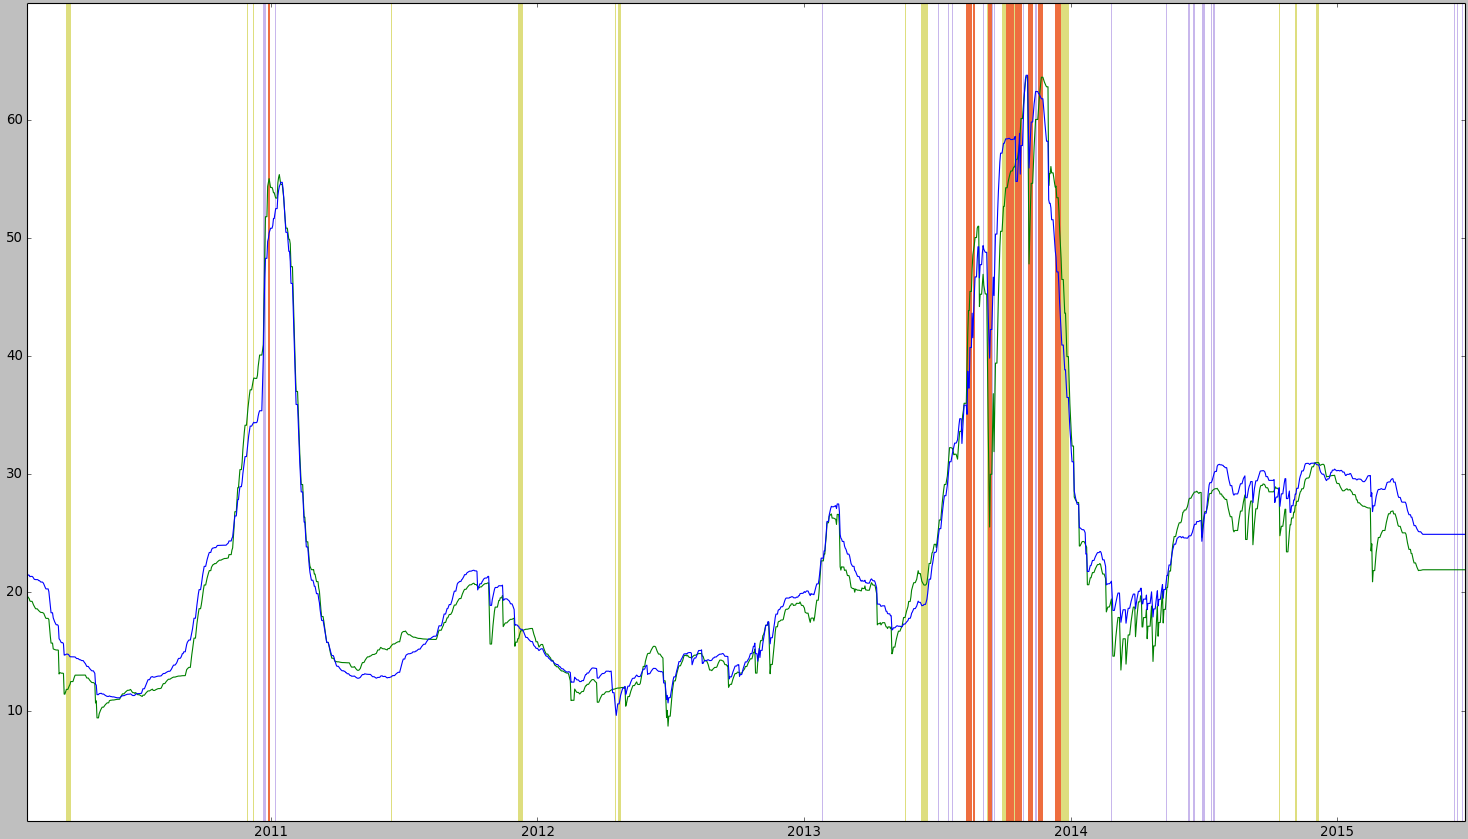
\includegraphics[width=1.1\textwidth]{graphs/RvsAvg_Whole.png}
		    	\caption{System Result (Green line - Centre Retail Price, Blue Line - Average Retail Price)}
		    	\label{fig:RvsR}
			\end{figure}
			
	
 \item Retail Price vs Arrival Data
			
			\begin{figure}[H]
		    	\centering
  		    	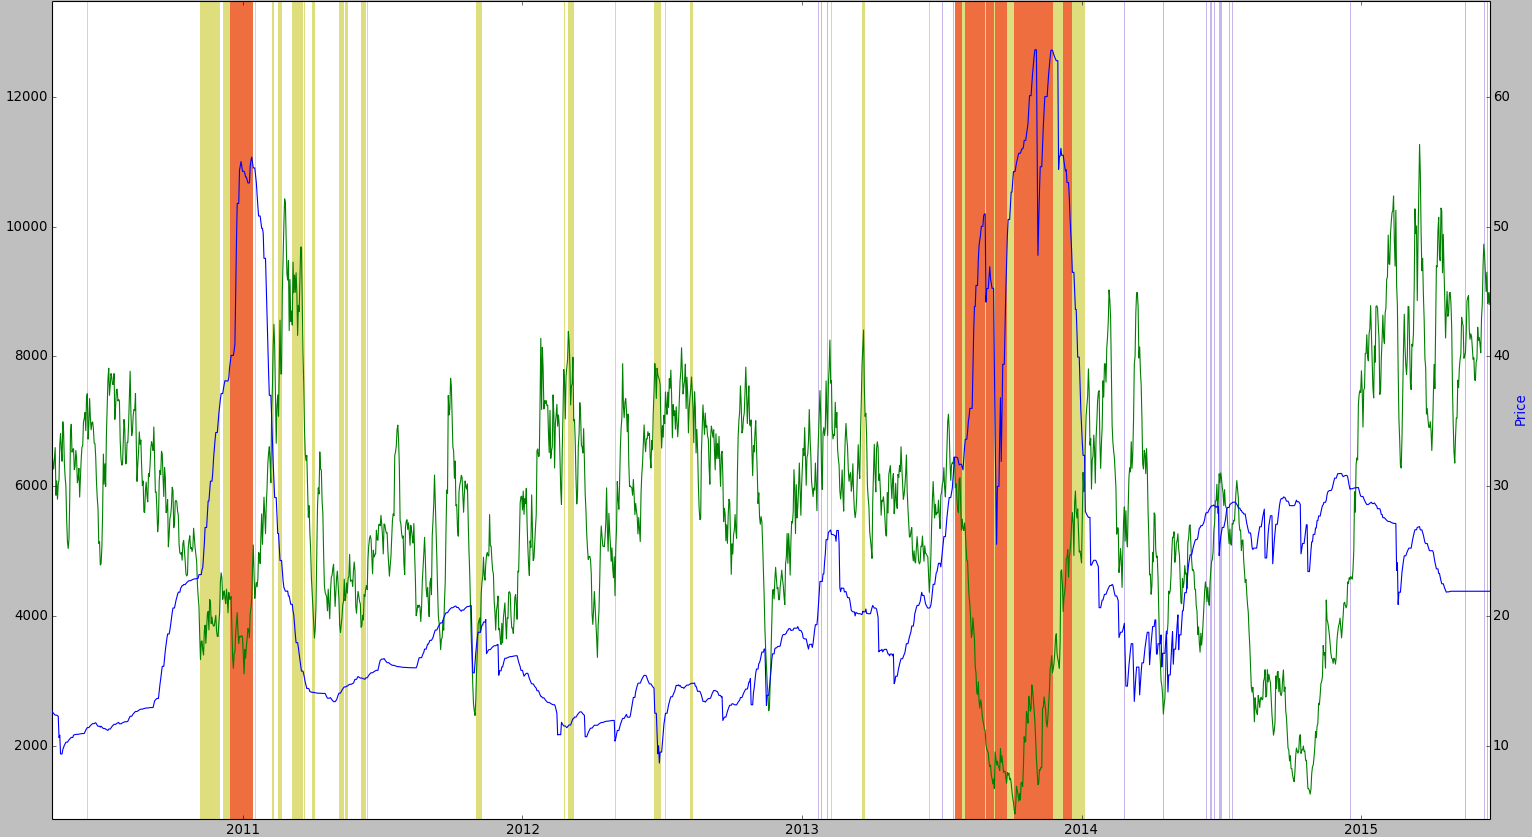
\includegraphics[width=1.1\textwidth]{graphs/RetailVsArrival_whole.png}
		    	\caption{System Result (Green line - Arrival Data of Onion, Blue Line - Retail Price)}
		    	\label{fig:RvsA}
			\end{figure}
			
	
 \item Retail Price vs Wholesale Price
			
			\begin{figure}[H]
		    	\centering
  		    	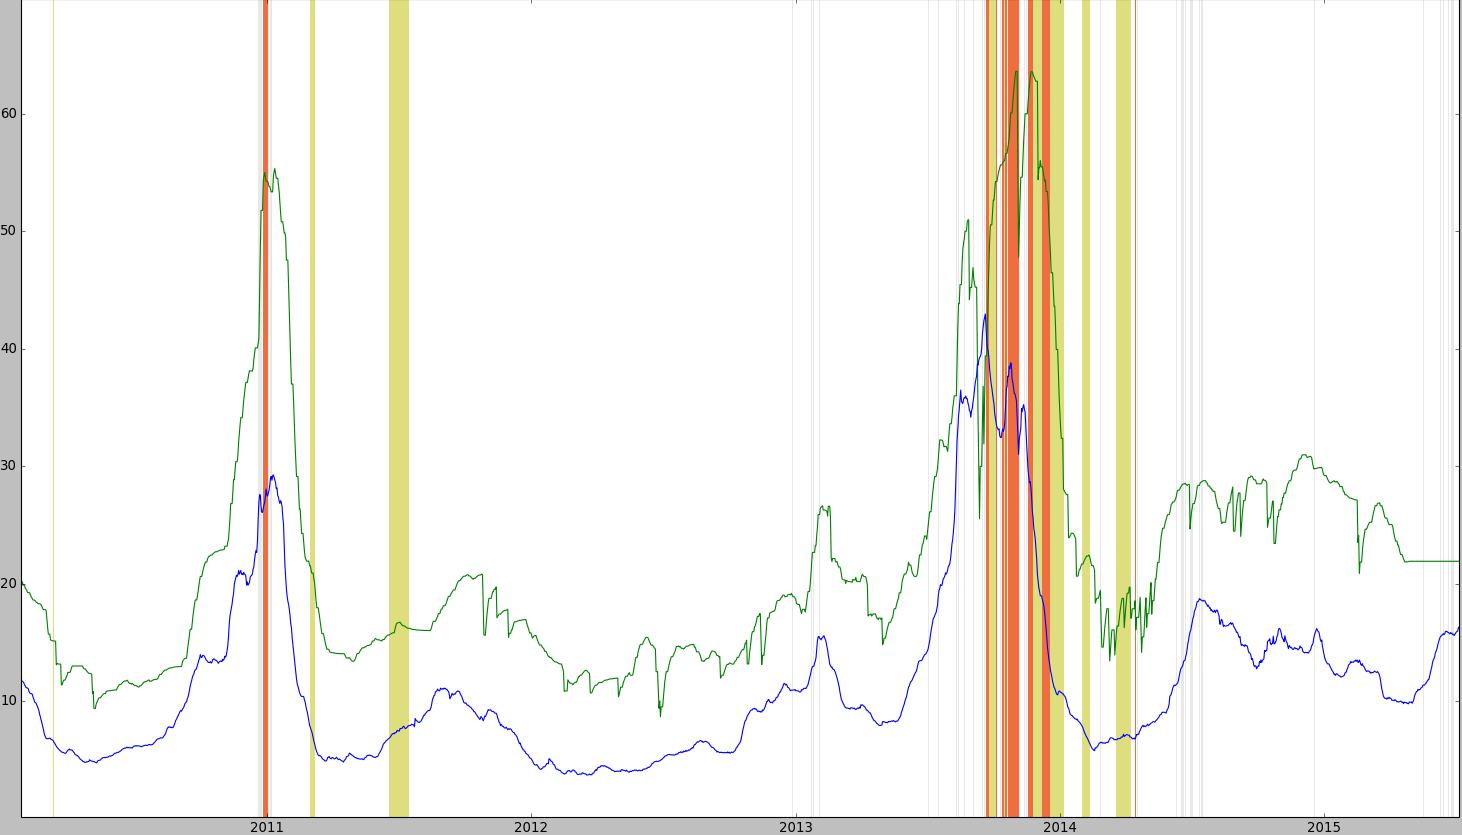
\includegraphics[width=1.1\textwidth]{graphs/retailVsWS_Whole.png}
		    	\caption{System Result (Green line - Retail Price, Blue Line - Wholesale Price)}
		    	\label{fig:RvsW}
			\end{figure}
			
	
 \item Wholesale Price vs Arrival Data
			
			\begin{figure}[H]
		    	\centering
  		    	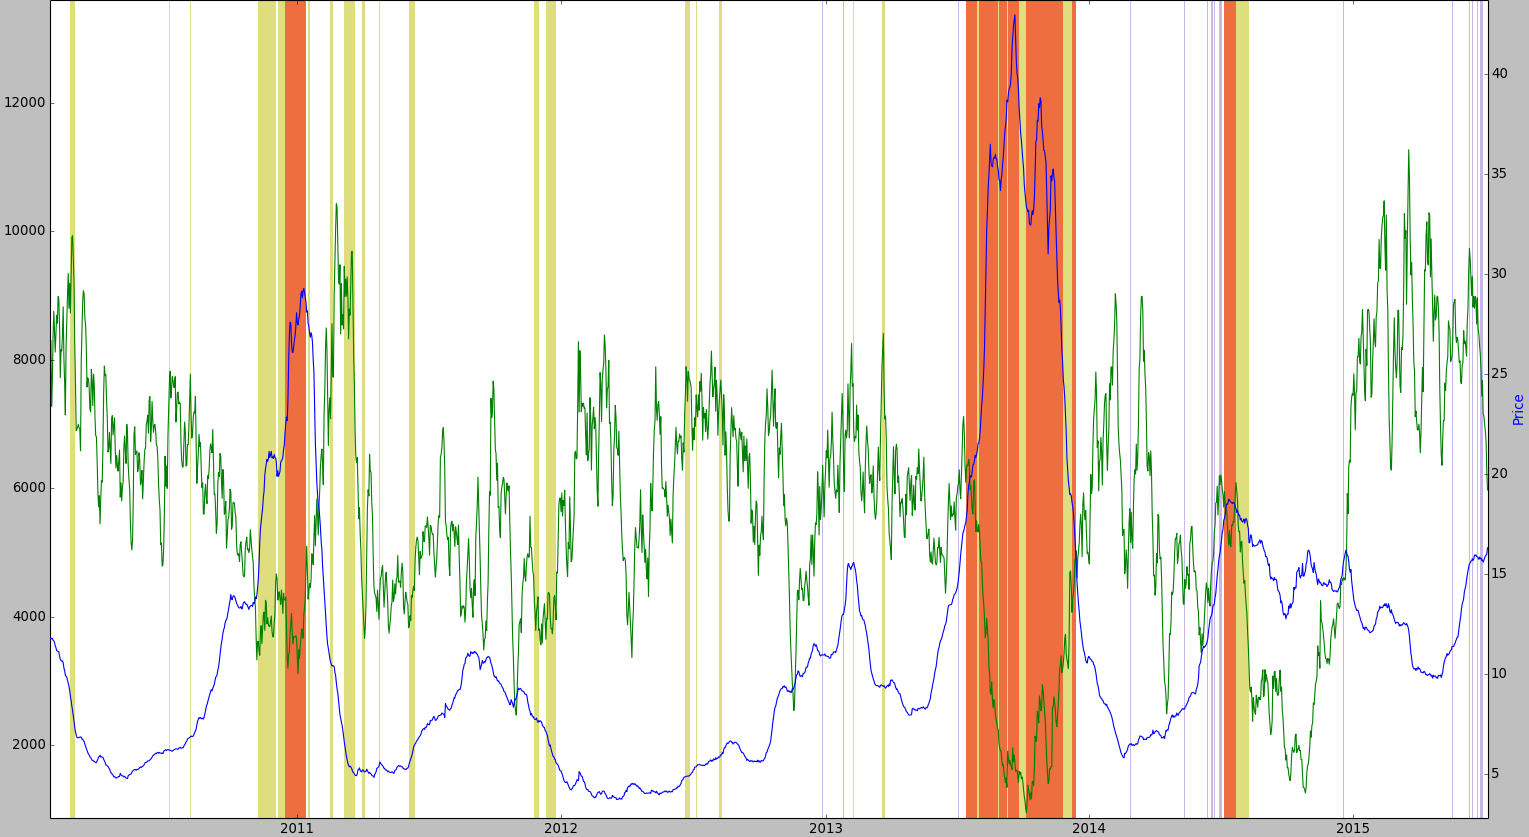
\includegraphics[width=1.1\textwidth]{graphs/WSvsArrival_Whole.png}
		    	\caption{System Result (Green line - Arrival Data of Onion, Blue Line - Wholesale Price)}
		    	\label{fig:WvsA}
			\end{figure}
			
	
\end{itemize}


Here are few examples comparing system results with the news articles and what news articles are saying about price hike.


\begin{table}[H]
\centering
\resizebox{\textwidth}{!}{
\begin{tabular}{|c|c|c|c|}
\hline
\textbf{System Reported Tenure} & \textbf{News Articles Link}                                                                                             & \textbf{Analysis Type} & \textbf{Location} \\ \hline
27-Dec-2010 to 29-Dec-2010      & http://timesofindia.indiatimes.com/city/pune/Onion-prices-still-leave-consumers-teary-eyed/articleshow/7147525.cms      & Retail vs Average      & Mumbai            \\ \hline
17-Oct-2013 to 27-Oct-2013      & http://www.thehindu.com/business/Industry/monopoly-of-wholesale-trade-causing-onion-price-hike/article5264512.ece       & Retail vs Average      & Mumbai            \\ \hline
15-Dec-2010 to 13-Jan-2011      & http://articles.economictimes.indiatimes.com/2010-12-21/news/27586208\_1\_minimum-export-price-onion-prices-mep         & Retail vs Arrival      & Mumbai            \\ \hline
17-Oct—2013 to 25-Nov-2013      & http://www.dnaindia.com/mumbai/report-dna-exclusive-traders-not-farmers-making-the-most-of-soaring-onion-price-1909850  & Retail vs Arrival      & Mumbai            \\ \hline
29-Jun-2014 to 06-July-2014     & http://timesofindia.indiatimes.com/india/Retail-onion-prices-soar-to-double-of-wholesale-rates/articleshow/37490678.cms & Retail vs Arrival      & Delhi             \\ \hline
18-Nov-2013 to 24-Nov-2013      & http://www.firstpost.com/politics/onion-tomato-price-hoardings-to-malign-party-cong-writes-to-ec-1238589.html           & Retail vs Wholesale    & Mumbai            \\ \hline
21-Oct-2013 to 04-Nov-2013      & http://www.dnaindia.com/mumbai/report-dna-exclusive-traders-not-farmers-making-the-most-of-soaring-onion-price-1909850  & Retail vs Wholesale    & Mumbai            \\ \hline
27-Oct-2013 to 03-Nov-2013      & http://www.thehindu.com/news/national/karnataka/are-farmers-benefiting-from-soaring-onion-prices/article5269250.ece     & Retail vs Wholesale    & Delhi             \\ \hline
17-Oct-2013 to 24-Nov-2013      & http://www.moneycontrol.com/news/economy/onion-prices-remain-high-at-rs-100kg-crisis-to-continue\_976318.html           & Wholesale vs Arrival   & Mumbai            \\ \hline
15-Dec-2010 to 12-Jan-2011      & http://articles.economictimes.indiatimes.com/2010-12-21/news/27586208\_1\_minimum-export-price-onion-prices-mep         & Wholesale vs Arrival   & Mumbai            \\ \hline
29-Jun-2014 to 05-July-2014     & http://timesofindia.indiatimes.com/india/Retail-onion-prices-soar-to-double-of-wholesale-rates/articleshow/37490678.cms & Wholesale vs Arrival   & Delhi             \\ \hline
\end{tabular}}

\caption{Few Examples}
\label{examples}

\end{table}


Few of the analysis which were local to center could not be matched with national news articles, but on digging more in regional news article, we could justify the anomaly. One of such case is the anomaly reported on 7th and 8th January 2013, in Delhi, for which news was reported in \href{http://www.jagran.com/news/business-onion-price-affected-from-fog-9987751.html}{Jagran local news paper} on 28th December 2012 which says due to fog there was disruption in the supply of onions. Despite of the speculation on low arrival of onion we observed considerable hike in arrival (which could be hoarded onion stocks brought into market) to earn better profits to take advantage of increased price of onion. Also, we have observed 2 news articles suspecting traders' nexus as the reason for the increased onion prices.


			\begin{figure}[H]
		    	\centering
  		    	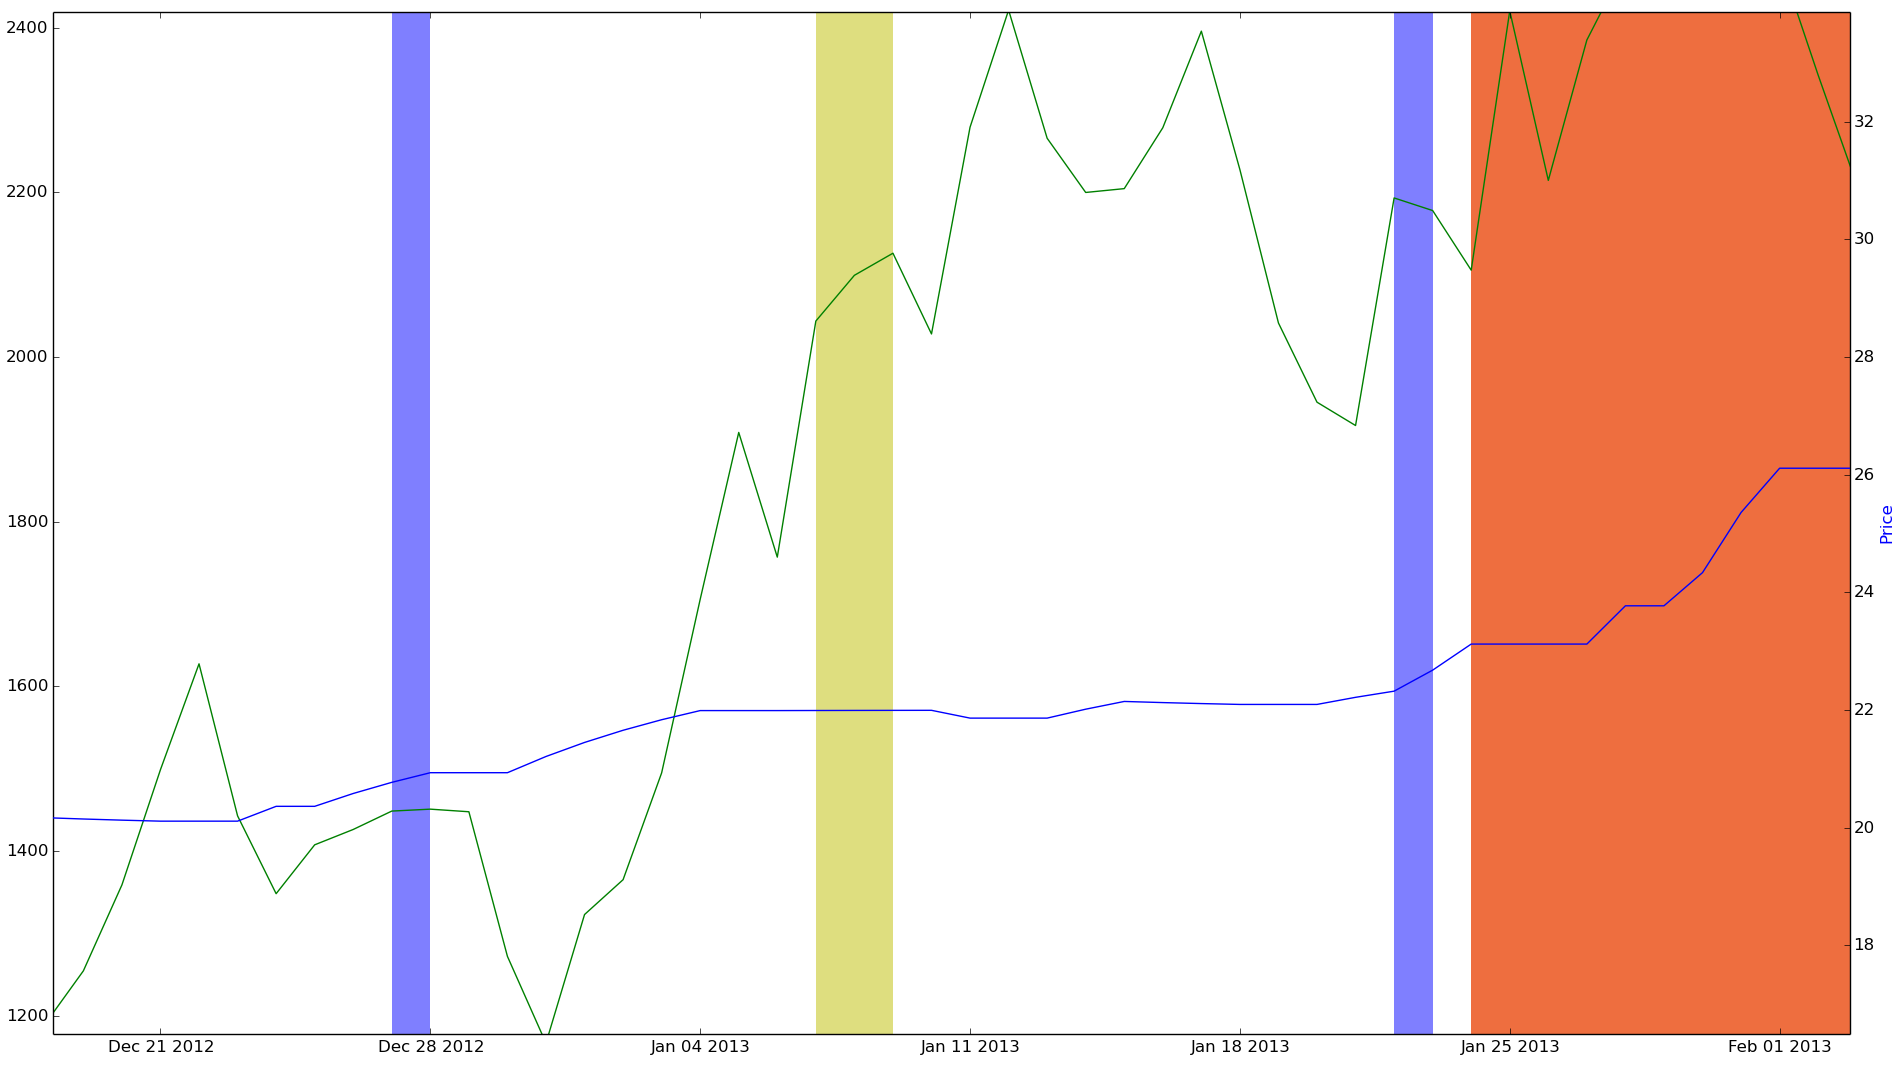
\includegraphics[width=1.1\textwidth]{graphs/localDelhiRegionalNewsPlusNexus.png}
		    	\caption{System Result (Green line - Arrival Data of Onion, Blue Line - Retail Price)}
		    	\label{fig:localExample}
			\end{figure}
			
News Article stated the following,

		\begin{figure}[H]
		    	\centering
  		    	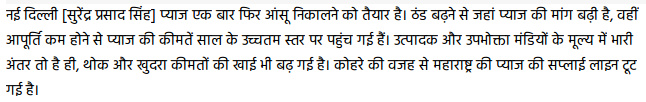
\includegraphics[width=1.1\textwidth]{graphs/localDelhiFog.png}
		    	\caption{Jagran News paper article}
		    	\label{fig:localDelhiFog}
		\end{figure}
\end{document}   